\documentclass{ctexart}
\usepackage{graphicx}
\usepackage{caption}
\usepackage{float}
\usepackage{amsmath}
\usepackage{fancyhdr}
\usepackage{xunicode-addon}
\usepackage{booktabs}
\usepackage{listings}
\usepackage{hyperref}
\usepackage[a4paper,hmargin=1.25in,vmargin=1in]{geometry}
% !TeX program = xelatex
\lstdefinestyle{mystyle}{
  basicstyle=\ttfamily\footnotesize,
  breakatwhitespace=false,         
  breaklines=true,                 
  captionpos=b,                    
  keepspaces=true,                 
  numbers=left,                    
  numbersep=5pt,                  
  showspaces=false,                
  showstringspaces=false,
  showtabs=false,                  
  tabsize=2
}

\lstset{style=mystyle}

\title{\begin{figure}[H]
	\centering 
	\includegraphics[height=7cm,width=14cm]{E:/Pictures/中科大.jpg}
	\end{figure}\Huge\textbf{数据结构实验报告1}\\\huge{一元多项式运算器}}
\date{}
\punctstyle{banjiao} 
\pagestyle{fancy}
	\fancyhead[C]{\LARGE\textbf{实验报告1}}
	\fancyhead[L]{}
	\fancyhead[R]{}
	\fancyfoot[C]{\thepage}
\begin{document}
	\maketitle
	\thispagestyle{empty}
	
	\[\makebox{\Large{姓名:\underline{\makebox[5cm]{高茂航}}}}\]
	
    \[\makebox{\Large{学号:\underline{\makebox[5cm]{PB22061161}}}}\]
	
	\[\makebox{\Large{日期:\underline{\makebox[5cm]{2023年10月15日}}}}\]
	
	\clearpage

	\pagenumbering{arabic}

	\section{问题描述}

	1.输入并创建多项式(按指数降序排列,系数浮点型,指数整型)(由于一开始没有考虑指数小于0的情况,且发现该情况除了积分与大于0的情况基本相同,
	因此不另外补充,另外由于后面有链表节点的插入函数,因此在创建链表时直接运用尾插法并要求指数降序排列);

2. 输出多项式,项数+每项系数指数(按指数升序或降序排列);

3.清空、销毁、清空、修改(插入新的结点、删除已有结点、修改已有结点的系数)多项式链表;

4. 实现多项式的加法、减法、求值、乘法和乘方、除法、四则运算,求微分(N阶导数)、不定积分、定积分。

	\section{算法描述}

	\subsection{数据结构}
	1.多项式用带头结点的单链表表示,多项式的项数存放在头结点;

	2.用指针数组存放N个多项式的头指针。
	\begin{lstlisting}[language=C, caption=头指针数组]
		Node* headlist[2];
		int i;
		printf("现在开始创建%d个多项式链表\n",LinkNum);
		for(i=0;i<LinkNum;i++){
			headlist[i]=Create();
			Print(headlist[i]);
		}
	\end{lstlisting}
	\begin{lstlisting}[language=C, caption=创建多项式链表结构过程]
		Node* Create(){//尾插法创建多项式链表,头节点指数域存多项式项数,每项次数不小于0
			Node *p=NULL,*head=NULL,*rear=NULL;
			int i,n;
			printf("请输入多项式项数");
			scanf("%d",&n);
			head=(Node*)malloc(sizeof(Node));
			head->coefficient=0;
			head->next=NULL;
			rear=head;
			if(n){
				printf("请依次输入多项式系数(浮点型)与指数(整型,降序排列且不小于0)");
				for(i=0;i<n;i++){
					p=(Node*)malloc(sizeof(Node));
					scanf("%f%d",&p->coefficient,&p->exponent);
					if(p->exponent>=0&&rear!=head&&p->exponent>rear->exponent){
						printf("项要降幂排列\n");
						break;
					}
					else if(p->exponent<0){
						printf("项的次数不能小于零\n");
						break;
					}
					else{
						rear->next=p;
						rear=p;
						rear->next=NULL;
					}
				}
				head=DeleteZero(head);
			}
			else
				head->exponent=0;
			return head;
		}
	\end{lstlisting}
	\subsection{程序结构}
	\begin{lstlisting}[language=C, caption=程序结构]
		void printMenu();//打印菜单
		void clearCache();//清除缓冲区无用数据
		Node* Create();//创建多项式链表
		Node* reCreate(Node*);//重建多项式链表
		void Print(Node*);//打印多项式链表
		Node* Addition(Node*,Node*);//多项式加法
		Node* Subtraction(Node*,Node*);//多项式减法
		void Evaluate(Node*);//多项式求值
		float Evaluate2(Node*,float);//已知未知数的多项式求值
		Node* Clear(Node*);//多项式链表清空
		void Destroy(Node* &);//多项式链表销毁
		void Modify(Node* &);//多项式修改
		void InsertNode(Node* &);//插入节点
		void DeleteNode(Node* &);//删除节点
		void ModifyNode(Node* &);//修改节点
		Node* Differential(Node*);//多项式微分
		Node* Derivation(Node*);//多项式求高阶导
		Node* Indefinite_Integral(Node*);//多项式不定积分
		void Definite_Integral(Node*);//多项式定积分
		Node* Multiplication(Node*,Node*);//多项式乘法
		Node* Exponentiation(Node*);//多项式乘方
		Node* DeleteZero(Node*);//把系数为0的非零节点删除
		Node* AddZero(Node*);//把稀疏多项式中缺少的次数用0补齐
		void Division(Node*,Node*);//多项式除法
		Node* NewDivision(Node*,Node*);//舍去余式的多项式除法
		void Arithmetic(Node*,Node*);//实现给定的多项式四则运算,除法不保留余式
		int main() {
			char ch;
			Node* headlist[2];
			int i;
			printf("现在开始创建%d个多项式链表\n",LinkNum);
			for(i=0;i<LinkNum;i++){
				headlist[i]=Create();
				Print(headlist[i]);
			}
			while (1) {
				printMenu();
				printf("请选择对应功能的序号:");
				scanf("%c", &ch);
				clearCache();
				if (ch == 'q')
					break;
				switch (ch) {
					case'a':{//多项式加法
						int i,j;
						scanf("%d%d",&i,&j);//输入进行运算的多项式序号
						Print(Addition(headlist[i-1],headlist[j-1]));
						break;
					}
					case'b':{//多项式减法
						int i,j;
						scanf("%d%d",&i,&j);//输入进行运算的多项式序号
						Print(Subtraction(headlist[i-1],headlist[j-1]));
						break;
					}
					case'c':{//多项式求值
						int i;
						scanf("%d",&i);//输入进行运算的多项式序号
						Evaluate(headlist[i-1]);
						break;
					}
					case'd':{//多项式修改
						int i;
						scanf("%d",&i);//输入进行修改的多项式序号
						Modify(headlist[i-1]);
						break;
					}
					case'e':{//多项式求导
						int i;
						scanf("%d",&i);//输入求导的多项式序号
						Print(Derivation(headlist[i-1]));
						break;
					}
					case'f':{//多项式不定积分
						int i;
						scanf("%d",&i);//输入求不定积分的多项式序号
						Print(Indefinite_Integral(headlist[i-1]));
						printf("+C(常数)\n");
						break;
					}
					case'g':{//多项式定积分
						int i;
						scanf("%d",&i);//输入求定积分的多项式序号
						Definite_Integral(headlist[i-1]);
						break;
					}
					case'h':{//多项式乘法
						int i,j;
						scanf("%d%d",&i,&j);//输入进行运算的多项式序号
						Print(Multiplication(headlist[i-1],headlist[j-1]));
						break;
					}
					case'i':{//多项式乘方
						int i;
						scanf("%d",&i);//输入求乘方的多项式序号
						Print(Exponentiation(headlist[i-1]));
						break;
					}
					case'j':{//多项式除法
						int i,j;
						scanf("%d%d",&i,&j);//输入进行运算的多项式序号
						Division(headlist[i-1],headlist[j-1]);
						break;
					}
					case'k': {//多项式四则运算
						Arithmetic(headlist[0],headlist[1]);
						break;
					}
					case'l':{//多项式链表清空重建
						int i;
						scanf("%d",&i);//输入需要清空重建的多项式序号
						Print(Clear(headlist[i-1]));
						Print(reCreate(Clear(headlist[i-1])));
						break;
					}
					default:
						break;
				}
			}
			for(i=0;i<LinkNum;i++)
				Destroy(headlist[i]);
			return 0;
		}
	\end{lstlisting}
	\subsubsection{主要功能算法}
	1.打印多项式链表成形如5x\^{}3+(-x\^{}2)+1的形式,注意考虑到系数为0、1和负数时特殊的打印方式。

	\begin{lstlisting}[language=C, caption=打印多项式链表]
	void Print(Node *head) {
			if(head){
				Node *p=head;
				printf("多项式有%d项",p->exponent);
				if(p->next){
					p=p->next;
					while(p&&p->next){
						if(!p->coefficient)
							p=p->next;
						else if(p->exponent>1){
							if(p->coefficient!=1&&p->coefficient>0){
								printf("%fx^%d+",p->coefficient,p->exponent);
								p=p->next;
							}
							else if(p->coefficient!=-1&&p->coefficient<0){
								printf("(%fx^%d)+",p->coefficient,p->exponent);
								p=p->next;
							}
							else if(p->coefficient==-1){
								printf("(-x^%d)+",p->exponent);
								p=p->next;
							}
							else{
								printf("x^%d+",p->exponent);
								p=p->next;
							}
						}
						else if(p->coefficient!=1&&p->coefficient>0){
							printf("%fx+",p->coefficient);
							p=p->next;
						}
						else if(p->coefficient==-1){
							printf("(-x)+");
							p=p->next;
						}
						else if(p->coefficient!=-1&&p->coefficient<0){
							printf("(%fx)+",p->coefficient);
							p=p->next;
						}
						else{
							printf("x+");
							p=p->next;
						}
					}
					if(p->exponent){
						if(p->exponent==1){
							if(p->coefficient!=-1&&p->coefficient<0)
								printf("(%fx)",p->coefficient);
							else if(p->coefficient==-1)
								printf("(-x)");
							else if(p->coefficient!=1&&p->coefficient>0)
								printf("%fx",p->coefficient);
							else
								printf("x");
						}
						else if(p->coefficient<0&&p->coefficient!=-1)
							printf("(%fx^%d)",p->coefficient,p->exponent);
						else if(p->coefficient==-1)
							printf("(-x^%d)",p->exponent);
						else if(p->coefficient!=1&&p->coefficient>0)
							printf("%fx^%d",p->coefficient,p->exponent);    
						else
							printf("x^%d",p->exponent);
					}
					else{
						if(p->coefficient>=0)
							printf("%f",p->coefficient);
						else if(p->coefficient<0)
							printf("(%f)",p->coefficient);
					}
				}
			}
			else
				printf("多项式无法打印");
		}
	\end{lstlisting}
	2.把系数为0的非零次节点删除,以免结果出现不符合常见形式的多项式,
	同时在这个函数里去零后再统计多项式项数更准确。
	\begin{lstlisting}[language=C, caption=删除系数为0的非零次项]
	Node* DeleteZero(Node* head){
		Node *p=head->next,*rear=head,*q=NULL;
		int i;
		while (p){
			if(!p->coefficient&&p->exponent){//把非零次项的0系数节点删除
				q=p;
				rear->next=p->next;
				p=p->next;
				free(q);
			}
			else if(rear!=head&&!p->coefficient&&!p->exponent){//把有非零系数的非零次项且末项为0的多项式末项删去
				rear->next=NULL;
				q=p;
				free(q);
				p=NULL;
			}
			else{//当只有一项0时能得以保留
				p=p->next;
				rear=rear->next;
			}
		}
		i=0;
		p=head->next;
		while (p){//遍历得到多项式项数
			i++;
			p=p->next;
		}
		if(i){
			head->exponent=i;
			return head;
		}
		else{//将形如0x^3+0x^2的多项式去掉0系数项后还需补一个0,使其还有一项
			p=(Node*)malloc(sizeof(Node));
			p->coefficient=0;
			p->exponent=0;
			head->exponent=1;
			p->next=NULL;
			head->next=p;
			return head;
		}
	}
	\end{lstlisting}
	3.加法(减法同理)。为了不破坏原链表,和多项式用一个新链表储存。两个指针分别指向两个多项式最高次项,
	依次移动两个指针并比较两个指针指向的次数,按多项式加法的规则进行运算。
	\begin{lstlisting}[language=C, caption=加法]
	Node* Addition(Node* head1,Node* head2){
		if(!head1||!head2){
			printf("\n进行加法运算的多项式不能没有项\n");
			return NULL;
		}
		Node *node=(Node*)malloc(sizeof(Node)),*p=head1->next,*q=head2->next,*rear=NULL,*pt=NULL;
		int i=0;
		node->next=NULL;
		pt=node;
		while(p&&q){
			if(p->exponent>q->exponent){
				rear=(Node*)malloc(sizeof(Node));
				rear->coefficient=p->coefficient;
				rear->exponent=p->exponent;
				p=p->next;
			}
			else if(q->exponent>p->exponent){
				rear=(Node*)malloc(sizeof(Node));
				rear->coefficient=q->coefficient;
				rear->exponent=q->exponent;
				q=q->next;
			}
			else{
				rear=(Node*)malloc(sizeof(Node));
				rear->coefficient=p->coefficient+q->coefficient;
				rear->exponent=q->exponent;
				q=q->next;
				p=p->next;
			}
			pt->next=rear;
			pt=rear;
			pt->next=NULL;
		}
		while(!p&&q){
			rear=(Node*)malloc(sizeof(Node));
			rear->coefficient=q->coefficient;
			rear->exponent=q->exponent;
			q=q->next;
			pt->next=rear;
			pt=rear;
			pt->next=NULL;
		}
		while(!q&&p){
			rear=(Node*)malloc(sizeof(Node));
			rear->coefficient=p->coefficient;
			rear->exponent=p->exponent;
			p=p->next;
			pt->next=rear;
			pt=rear;
			pt->next=NULL;
		}
		node=DeleteZero(node);
		return node;
	}
	\end{lstlisting}

	4.多项式求值:遍历链表,代码略。

	5.多项式链表销毁与清空:设置前驱指针,依次释放每个节点的内存,代码略。

	6.链表节点插入、删除与修改:设置前驱指针并遍历链表,分情况讨论。
	\begin{lstlisting}[language=C, caption=链表节点插入、删除与修改]
		void InsertNode(Node* &head){//插入节点
    if(!head)
        printf("\n进行插入的多项式不能没有项\n");
    else{
        Node *p=head->next,*node=NULL;
        float coef;
        int exp;
        printf("请输入要插入节点的系数(浮点型)和指数(整型)");
        scanf("%f%d",&coef,&exp);
        if(!p){
            head->next=node;
            node->coefficient=coef;
            node->exponent=exp;
            head->next->next=NULL;
            head->exponent++;
            return ;
        }
        while(p){
            if(p->exponent<exp){
                node=(Node*)malloc(sizeof(Node));
                node->next=p;
                head->next=node;
                node->coefficient=coef;
                node->exponent=exp;
                head->exponent++;
                return ;
            }
            else if(p->exponent>exp&&p->next->exponent>exp)
                p=p->next;
            else if(p->exponent>exp&&p->next->exponent<exp){
                node=(Node*)malloc(sizeof(Node));
                node->next=p->next;
                p->next=node;
                node->coefficient=coef;
                node->exponent=exp;
                head->exponent++;
                return ;
            }
            else if(p->exponent==exp)
                p->coefficient=p->coefficient+coef;
            else if(p->exponent>exp&&!p->next){
                node=(Node*)malloc(sizeof(Node));
                p->next=node;
                node->coefficient=coef;
                node->exponent=exp;
                p->next->next=NULL;
                head->exponent++;
                return ;
            }
        }
    }
}
void DeleteNode(Node* &head){//删除节点
    if(!head)
        printf("\n进行插入的多项式不能没有项\n");
    else{
        Node *p=head->next,*prior=head;
        int exp;
        printf("请输入要删除节点的指数(整型)");
        scanf("%d",&exp);
        while(p){
            if(p->exponent==exp){
                prior->next=p->next;
                free(p);
                head->exponent--;
                return ;
            }
            p=p->next;
            prior=prior->next;
        }
        printf("找不到要删除指数对应的项");
        return ;
    }
}
	\end{lstlisting}
7.多项式求微分并把结果储存到一个新链表,关键为遍历修改多项式每一项(积分同理),求高阶导就是反复调用求微分的函数。
	\begin{lstlisting}[language=C, caption=多项式微分]
	Node* Differential(Node* head){
		if(!head){
			printf("\n进行求微分运算的多项式不能没有项\n");
			return NULL;
		}
		Node* node=(Node*)malloc(sizeof(Node)),*rear=NULL,*q=NULL,*p=head->next;
		int i;
		q=node->next;
		rear=node;
		for(i=0;i<head->exponent&&p->exponent;i++){
			q=(Node*)malloc(sizeof(Node));
			q->coefficient=p->coefficient*p->exponent;
			q->exponent=p->exponent-1;
			rear->next=q;
			rear=q;
			rear->next=NULL;
			p=p->next;
		}
		node=DeleteZero(node);
		return node;
	}
	\end{lstlisting}
	\begin{lstlisting}[language=C, caption=]
		8.多项式乘法并把结果储存到一个新链表,算法是将第一个多项式的每一项乘第二个多项式后得到的多项式相加得到结果。求乘方就是反复调用乘法函数。
	Node* Multiplication(Node* head1,Node* head2){
		if(!head1||!head2){
			printf("\n进行乘法运算的多项式不能没有项\n");
			return NULL;
		}
		Node *node=NULL,*p=head1,*q=head2->next,*list[head1->exponent];
		int i;
		for(i=0;i<head1->exponent;i++){
			p=p->next;
			list[i]=(Node*)malloc(sizeof(Node));
			list[i]->exponent=head2->exponent;
			Node *rear=NULL,*pt=list[i];
			while (q){
				rear=(Node*)malloc(sizeof(Node));
				rear->exponent=p->exponent+q->exponent;
				rear->coefficient=p->coefficient*q->coefficient;
				q=q->next;
				pt->next=rear;
				pt=rear;
				pt->next=NULL;
			}
			q=head2->next;
		}
		for(i=1;i<head1->exponent;i++)//将指针数组里的多项式累加得到结果
			list[i]=Addition(list[i-1],list[i]);
		node=list[head1->exponent-1];
		node=DeleteZero(node);
		return node;
	}
	\end{lstlisting}
	9.实现多项式除法,首先要把被除式中缺少的次数用0补齐,利用被除式=除式*商式+余式,进入循环条件是中间余式次数高于除式。
	\begin{lstlisting}[language=C, caption=多项式除法]
	void Division(Node* head1,Node* head2){
    if(!head1||!head2)
        printf("\n进行除法运算的多项式不能没有项\n");
    else{
        Node *Dividend=AddZero(head1),*Divisor=DeleteZero(head2);
        if(!Divisor->next->coefficient)
            printf("除数不能为零!");
        Node *Remainder=Dividend,*Quotient=(Node*)malloc(sizeof(Node)),*p=NULL,*rear=NULL;//Dividen表示被除式指针,Divisor表示除式指针,Quotient表示商式指针,Remainder表示余式指针
        rear=Quotient;
        rear->exponent=1;//首先把商式置为0
        rear->next=NULL;
        p=(Node*)malloc(sizeof(Node));
        p->coefficient=0;
        p->exponent=0;
        rear->next=p;
        rear=p;
        rear->next=NULL;
		Remainder=Subtraction(Remainder,Multiplication(Quotient,Divisor));
        while (Remainder->next->exponent>Divisor->next->exponent){//余式次数高于除式,进入循环
            Node* pt=Remainder->next;
            if(!rear->coefficient&&!rear->exponent){//初始状态商式为0时
                rear->coefficient=pt->coefficient/Divisor->next->coefficient;
                rear->exponent=pt->exponent-Divisor->next->exponent;
            }
            else{
                p=(Node*)malloc(sizeof(Node));
                p->coefficient=pt->coefficient/Divisor->next->coefficient;
                p->exponent=pt->exponent-Divisor->next->exponent;
                rear->next=p;
                rear=p;
                rear->next=NULL;
            }
            Node *temp=(Node*)malloc(sizeof(Node));//temp的内容为商式的最后一项
            temp->exponent=1;
            temp->next=(Node*)malloc(sizeof(Node));
            temp->next->coefficient=rear->coefficient;
            temp->next->exponent=rear->exponent;
            temp->next->next=NULL;
            Remainder=Subtraction(Remainder,Multiplication(temp,Divisor));
        }
		if(Remainder->next->exponent==Divisor->next->exponent){//余式次数等于除式
			Node* pt=Remainder->next;
            if(!rear->coefficient&&!rear->exponent){
                rear->coefficient=pt->coefficient/Divisor->next->coefficient;
                rear->exponent=pt->exponent-Divisor->next->exponent;
            }
            else{
                p=(Node*)malloc(sizeof(Node));
                p->coefficient=pt->coefficient/Divisor->next->coefficient;
                p->exponent=pt->exponent-Divisor->next->exponent;
                rear->next=p;
                rear=p;
                rear->next=NULL;
            }
            Node *temp=(Node*)malloc(sizeof(Node));
            temp->exponent=1;
            temp->next=(Node*)malloc(sizeof(Node));
            temp->next->coefficient=rear->coefficient;
            temp->next->exponent=rear->exponent;
            temp->next->next=NULL;
            Remainder=Subtraction(Remainder,Multiplication(temp,Divisor));
		}
        Quotient=DeleteZero(Quotient);
        Print(Quotient);//商式
        Remainder=DeleteZero(Remainder);
        Print(Remainder);//余式
    }
}
Node* AddZero(Node* head){//把稀疏多项式中缺少的次数用0补齐
    Node *p=head->next,*rear=NULL;
    while(p){
        if(p->next&&p->next->exponent!=p->exponent-1){
            rear=(Node*)malloc(sizeof(Node));
            rear->coefficient=0;
            rear->exponent=p->exponent-1;
            rear->next=p->next;
            p->next=rear;
        }
        else if(!p->next&&p->exponent){
            rear=(Node*)malloc(sizeof(Node));
            rear->coefficient=0;
            rear->exponent=p->exponent-1;
            p->next=rear;
			p->next->next=NULL;
        }
        p=p->next;
    }
    p=head->next;
    int i=0;
    while (p){
        i++;
        p=p->next;
    }
    head->exponent=i;
    return head;
}
	\end{lstlisting}
	10.实现多项式四则运算。本来想用多项式的序号代替多项式进行四则运算,如(1+2)*3表示(1式+2式)*3式,
	进而需要用栈和逆波兰表示法表示(1+2)*3,但后来发现序号的运算不能代替多项式的运算,
	因此没能实现对任意输入的多项进行式四则运算(仍用输入(1+2)*3表示(1式+2式)*3式),有待探究。
	\begin{lstlisting}[language=C, caption=给定的多项式四则运算]
	void Arithmetic(Node* head1,Node* head2){
		printf("(1式+2式)*1式/2式后");
		Print(NewDivision(Multiplication(Addition(head1,head2),head1),head2));
	}
	\end{lstlisting}
	
	\section{调试分析}
	调试中遇到的主要bug是Segmentation fault,产生原因主要是以下三点:

	1.指针未初始化为NULL就解引用;

	2.创建链表时尾指针没有指向NULL(尾插法不熟练导致);

	3.修改链表系列函数的参数一开始不是指针引用而只是指针,这样会导致头指针指向未知的位置,导致接下来调用其他函数时出错。

另外,还出现内存申请失败的异常,后来发现是指针指向出现问题,原因和上面的bug大同小异。
	\section{算法时空分析}
	1.储存多项式的链表空间复杂度是$O(n)$;

	2.创建、加、减、增、删、改、微分、积分运算的时间复杂度为$O(n)$;
	
	3.乘法运算的时间复杂度为$O(n^2)$,除法运算的时间复杂度为$O(n^3)$。
	\section{测试结果分析}
	\begin{figure}[H]
		\centering 
		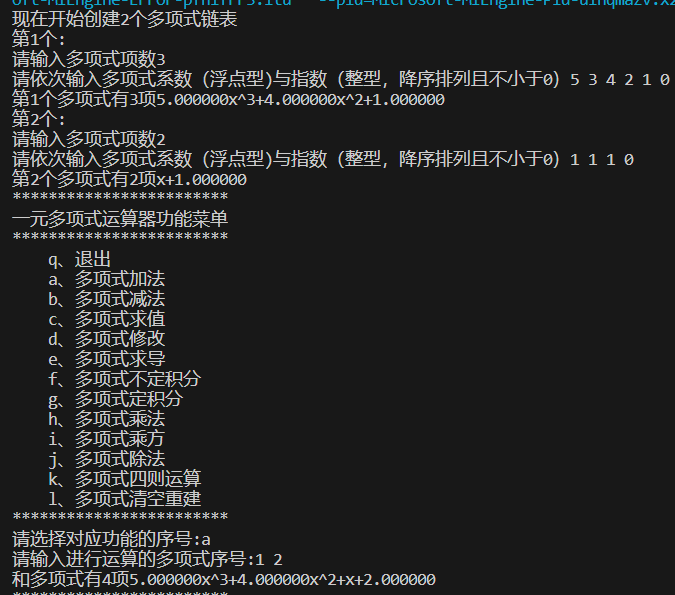
\includegraphics[height=10cm,width=14cm]{1.png}
		\end{figure}
		\begin{figure}[H]
		\centering 
		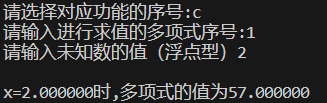
\includegraphics[height=2cm,width=6cm]{2.png}
		\end{figure}
		\begin{figure}[H]
		\centering 
		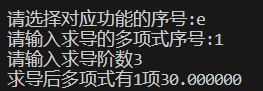
\includegraphics[height=2cm,width=6cm]{4.png}
		\end{figure}
		\begin{figure}[H]
		\centering 
		
\includegraphics[height=1.5cm,width=12cm]{5.png}
		\end{figure}
		\begin{figure}[H]
		\centering 
		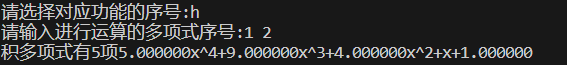
\includegraphics[height=1.5cm,width=12cm]{6.png}
		\end{figure}
		\begin{figure}[H]
		\centering 
		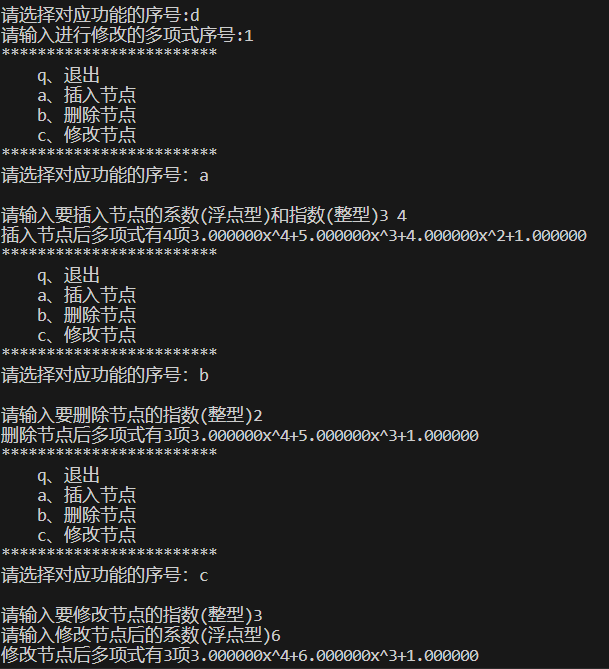
\includegraphics[height=12cm,width=12cm]{3.png}
		\end{figure}
		\begin{figure}[H]
		\centering 
		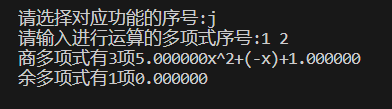
\includegraphics[height=4cm,width=14cm]{7.png}
		\end{figure}
		\begin{figure}[H]
		\centering 
		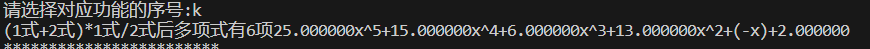
\includegraphics[height=1cm,width=14cm]{8.png}
		\end{figure}
	\section{实验体会收获}
		通过本次实验,进一步提高了链表操作的熟练程度,加深了对线性表结构的理解,
		为进一步学习其他数据结构打下基础。
\end{document}